\let\negmedspace\undefined
\let\negthickspace\undefined
\documentclass[journal]{IEEEtran}
\usepackage[a5paper, margin =  10mm, onecolumn]{geometry}
%\usepackage{lmodern} % Ensure lmodern is loaded for pdflatex
\usepackage{tfrupee} % Include tfrupee package

\setlength{\headheight}{1cm} % Set the height of the header box
\setlength{\headsep}{0mm}     % Set the distance between the header box and the top of the text

\usepackage{gvv-book}
\usepackage{gvv}
\usepackage{cite}
\usepackage{amsmath,amssymb,amsfonts,amsthm}
\usepackage{algorithmic}
\usepackage{graphicx}
\usepackage{textcomp}
\usepackage{xcolor}
\usepackage{txfonts}
\usepackage{listings}
\usepackage{enumitem}
\usepackage{mathtools}
\usepackage{gensymb}
\usepackage{comment}
\usepackage[breaklinks =  true]{hyperref}
\usepackage{tkz-euclide} 
\usepackage{listings}
% \usepackage{gvv}                                        
\def\inputGnumericTable{}                                 
\usepackage[latin1]{inputenc}                                
\usepackage{color}                                            
\usepackage{array}                                            
\usepackage{longtable}                                       
\usepackage{calc}                                             
\usepackage{multirow}                                         
\usepackage{hhline}                                           
\usepackage{ifthen}                                           
\usepackage{lscape}
\begin{document}

\bibliographystyle{IEEEtran}
\vspace{3cm}

\title{2.10.63}
\author{EE25BTECH11034 - Kishora Karthik}
% \maketitle
% \newpage
% \bigskip
{\let\newpage\relax\maketitle}

\renewcommand{\thefigure}{\theenumi}
\renewcommand{\thetable}{\theenumi}
%\setlength{\intextsep}{10pt} % Space between text and floats
\textbf{Question:}\\
A vector $\vec{A}$ has components $A_1, A_2, A_3$ in a right-handed rectangular Cartesian coordinate system $oxyz$. The coordinate system is rotated about the $x$-axis through an angle $\frac{\pi}{2}$. Find the components of $\vec{A}$ in the new coordinate system in terms of $A_1, A_2, A_3$.\\
\textbf{Solution:}\\
In the original coordinate system $S$,
\begin{align}
    \vec{A_S} = \myvec{ A_1 \\ A_2 \\ A_3}  
\end{align}
Let the new coordinate system be $S'$, obtained by rotating $S$ about the $x$-axis by an angle $\theta = \frac{\pi}{2}$. The components of the same vector $\vec{A}$ in the new system are,
\begin{align}
    \myvec{A'_1 \\ A'_2 \\ A'_3}   = R \myvec{A_1 \\ A_2 \\ A_3} 
\end{align}
where $R$ is the rotation matrix.
For a rotation of the coordinate system by an angle $\theta$ about the $x$-axis, 
\begin{align}
    R_x(\theta) = \myvec{1 & 0 & 0 \\ 0 & \cos\theta & \sin\theta \\ 0 & -\sin\theta & \cos\theta}  
\end{align}
Given, $\theta = \frac{\pi}{2}$.So,
\begin{align}    
R = \myvec{ 1 & 0 & 0 \\ 0 & \cos(\frac{\pi}{2}) & \sin(\frac{\pi}{2}) \\ 0 & -\sin(\frac{\pi}{2}) & \cos(\frac{\pi}{2})}   = \myvec{ 1 & 0 & 0 \\ 0 & 0 & 1 \\ 0 & -1 & 0}  
\end{align}
\begin{align}
    \myvec{A'_1 \\ A'_2 \\ A'_3}  = \myvec{1 & 0 & 0 \\ 0 & 0 & 1 \\ 0 & -1 & 0}   \myvec{ A_1 \\ A_2 \\ A_3}  
\end{align}
\begin{align}
A'_1 &= (1 \cdot A_1) + (0 \cdot A_2) + (0 \cdot A_3) = A_1 \\
A'_2 &= (0 \cdot A_1) + (0 \cdot A_2) + (1 \cdot A_3) = A_3 \\
A'_3 &= (0 \cdot A_1) + (-1 \cdot A_2) + (0 \cdot A_3) = -A_2
\end{align}
\begin{align}
\implies \myvec{A'_1 \\ A'_2 \\ A'_3} =\myvec{ A_1 \\ A_3 \\ -A_2} 
\end{align}
$\therefore$ The components of the vector $\vec{A}$ in the new coordinate system are:
$A'_1 = A_1$, $A'_2 = A_3$ and $A'_3 = -A_2$.\\\\
    \centering   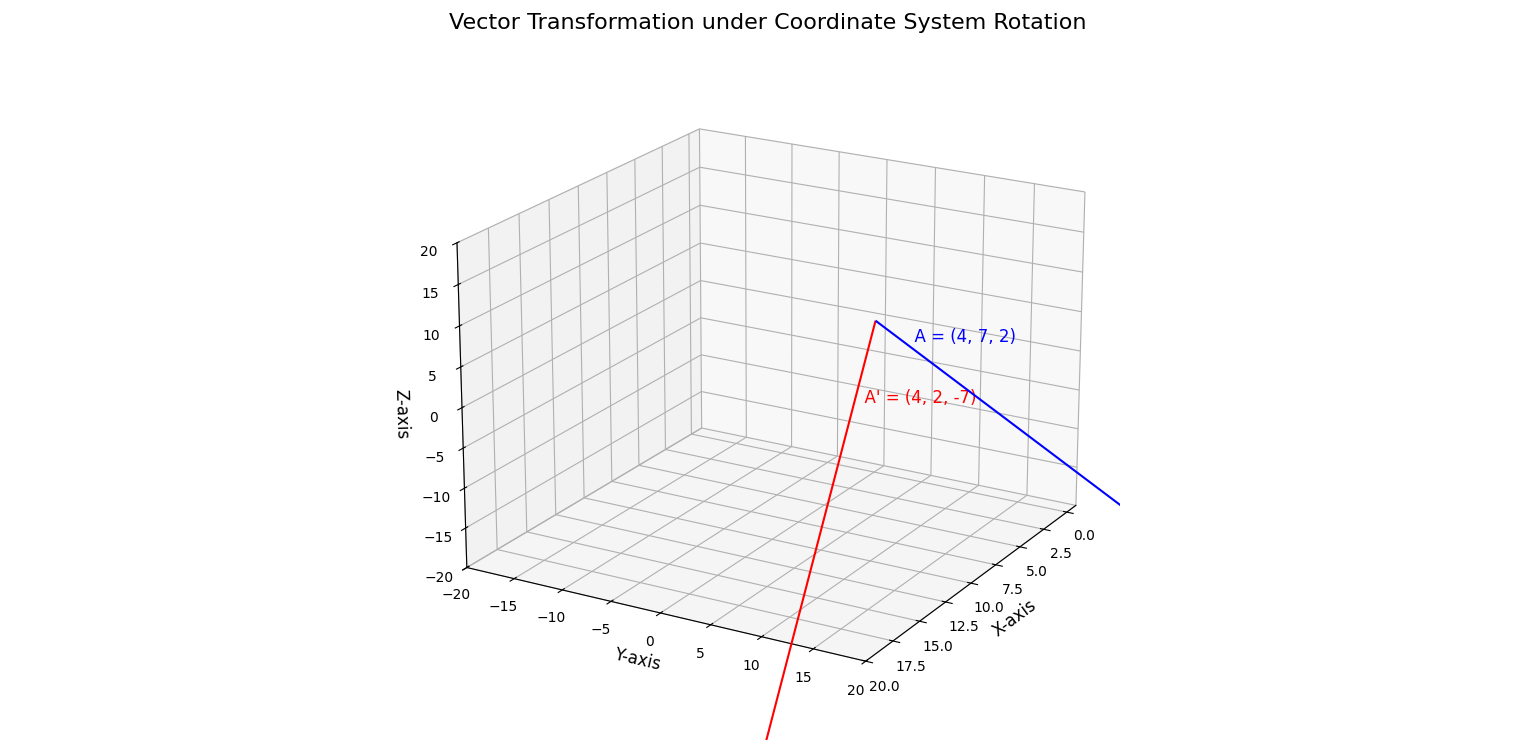
\includegraphics[width=\columnwidth, height=1\textheight, keepaspectratio]{figs/fig1.png} 
\end{document}
